% Intended LaTeX compiler: pdflatex
\documentclass[10pt,a4paper,UTF8]{article}
\usepackage{zclorg}
\author{emacsun}
\date{}
\title{曲线拟合过程中的欠定过定问题}
\hypersetup{
 pdfauthor={emacsun},
 pdftitle={曲线拟合过程中的欠定过定问题},
 pdfkeywords={},
 pdfsubject={},
 pdfcreator={Emacs 25.0.50.1 (Org mode 9.0.5)},
 pdflang={English}}
\begin{document}

\maketitle
\tableofcontents
\titlepic{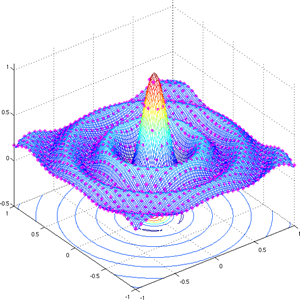
\includegraphics[scale=0.25]{../../img/sinc.PNG}}

\section{问题}
\label{sec:orged76f9a}


曲线拟合过程中,我们有目标函数
\begin{equation}
\label{eq:1}
y(x, \mathbf{w}) = w_{0} + w_{1}x + \ldots + w_{M}x^{M} = \sum_{j=0}^{M}w_{j}x^{j}
\end{equation}
误差函数:
\begin{equation}
\label{eq:2}
E( \mathbf{w}) = \frac{1}{2} \sum_{n=1}^{N}\{y(x_{n}, \mathbf{w}) - t_{n}\}^{2}
\end{equation}
对于这个问题,当训练数据集合小于\(w_{j}\)的个数时,我们可以认为对(\ref{eq:2})求导,求得\(w_{j}\)的过程为欠定方程的求解过程;当训练数据集合大于\(w_{j}\)的个数时,对(\ref{eq:2})求导,求得\(w_{j}\)的过程是过定方程的求解过程。

\section{抽象}
\label{sec:orgd418997}


不管是欠定还是过定,最小化 (\ref{eq:2})的解\(\mathbf{w} = \{w_{j}\}\)都是一般线性方程:\[\sum_{j=0}^{M}A_{ij}w_{j} = T_{i}\]的解。其中\(A_{ij} = \sum_{n=1}^{N}(x_{n})^{i+j}\),\(T_{i} = \sum_{n=1}^{N}(x_{n})^{i}t_{n}\)


我们可以把(\ref{eq:1})带入(\ref{eq:2}),得:
\begin{eqnarray}
\label{eq:3}
E( \mathbf{w})&=&\frac{1}{2} \sum_{n=1}^{N}\{ \sum_{j=0}^{M}w_{j}x_{n}^{j} - t_{n}\}^{2} \\
\end{eqnarray}

对于(\ref{eq:3}),我们求\(w_{i}\),则有:
\begin{eqnarray}
\label{eq:4}
\frac{dx}{dw_{i}}&=& \sum_{n=1}^{N} \{ \sum_{j=0}^{M}w_{j}x_{n}^{j} - t_{n} \}x_{n}^{i}   \\
&=& \sum_{n=1}^{N}\sum_{j=0}^{M}w_{j}x_{n}^{j} x_{n}^{i} - \sum_{n=1}^{N}t_{n}x_{n}^{i}
\end{eqnarray}

令(\ref{eq:4})等于零,我们得到关于\(w_{j},j=0,\ldots ,M\)的方程:
\begin{equation}
\label{eq:5}
\sum_{n=1}^{N}\sum_{j=0}^{M}w_{j}x_{n}^{j}x_{n}^{i} = \sum_{n=1}^{N}t_{n}x_{n}^{i}
\end{equation}

整理得到,
\begin{equation}
\label{eq:6}
\sum_{j=0}^{M}w_{j} \sum_{n=1}^{N} x_{n}^{i+j} = \sum_{n=1}^{N}t_{n}x_{n}^{i}
\end{equation}

令\(A_{ij} = \sum_{n=1}^{N} x_{n}^{i+j}\),\(T_{i} = \sum_{n=1}t_{n}x_{n}^{i}\),所以我们得到了:
\[\sum_{j=0}^{M} A_{ij}w_{j}=T_{i} \]
\section{总结}
\label{sec:org330dd01}


我们看到,对于(\ref{eq:6}),可以扩展为\(M+1\)个方程,即:
\begin{eqnarray*}
\sum_{j=0}^{M} A_{0j}w_{j} &=&T_{0} \\
\sum_{j=0}^{M} A_{1j}w_{j} &=&T_{1} \\
\vdots &=& \vdots \\
\sum_{j=0}^{M} A_{Mj}w_{j} &=&T_{M}
\end{eqnarray*}
所以我们有\(M+1\)个方程\(M+1\)个未知数\(w_{j},j=0,\ldots ,M\)
\end{document}
